\documentclass[letter,11pt]{article}

\usepackage[spanish,es-nodecimaldot]{babel}
\usepackage[utf8]{inputenc}

\usepackage{lmodern}
\usepackage[T1]{fontenc}
\usepackage{textcomp}

\usepackage{framed}
\usepackage[svgnames]{xcolor}
\colorlet{shadecolor}{Gainsboro!50}

\usepackage[labelfont=bf]{caption}
\usepackage{graphicx}
\usepackage{pstricks}

\usepackage{anysize}
\marginsize{3cm}{2cm}{2cm}{3cm}

\usepackage{url}
\usepackage{siunitx}
\usepackage{amsmath}
\usepackage{array}
\usepackage{alltt}

\usepackage{caption}
\newcommand{\source}[1]{\vspace{-11pt} \caption*{\small{\textbf{Nota:} {#1}}}}

\usepackage{fancyhdr}
\usepackage{lastpage}
\pagestyle{fancy}
\fancyhf{}
\fancyhead[LE,RO]{Laboratorio de Física Básica II}
\fancyfoot[CO,CE]{\thepage\ de \pageref{LastPage}}

\special{papersize=215.9mm,279.4mm}

\usepackage[
    pdfauthor={Carlos Eduardo Caballero Burgoa},%
    pdftitle={Laboratorio de Física Básica II},%
    pdfsubject={Péndulo simple},%
    colorlinks,%
    citecolor=black,%
    filecolor=black,%
    linkcolor=black,%
    urlcolor=black,
    breaklinks]{hyperref}
\usepackage{breakurl}

\newcommand{\blankpage}{
\newpage
\thispagestyle{empty}
\mbox{}
\newpage
}

\renewcommand{\arraystretch}{1.2}

\title{Examen: Laboratorio Física II \\Péndulo simple}
\author{Carlos Eduardo Caballero Burgoa \\
    \small{\href{mailto:200201226@est.umss.edu}{200201226@est.umss.edu}}
}
\date{14 de julio de 2021}

\begin{document}

\maketitle
\begin{center}
    \textbf{Grupo}: Miércoles\\
    \textbf{Gestión}: I/2021\\
    \textbf{Docente}: Ing. Milka Mónica Torrico Troche\\
    \textbf{Carrera}: Ing. Electromecánica
\end{center}

\begin{abstract}
Este documento detalla el experimento realizado para hallar la
relación funcional entre el periodo de oscilación ($T$) y la longitud ($L$) de
un péndulo simple, además de calcular el valor de la aceleración de la gravedad;
para esto se realizó la medición de 5 oscilaciones de un péndulo con una
longitud determinada; y posteriormente se calcula la relación funcional después
de linealizar la curva y ajustarla con el método de mínimos cuadrados,
finalmente se determinó el valor de la gravedad, resultando ser igual a:
$(10.23 \pm 0.37)[m/s^2]; 3.63\%$.
\end{abstract}

\section{Introducción}

Un péndulo simple es un modelo idealizado que consiste en una masa puntual
suspendida de una cuerda no expansible y de masa despreciable. Si la masa se
mueve a un lado de su posición de equilibrio vertical descendente, oscilará
alrededor de dicha posición \cite{Young&Freedman}.

\begin{figure}
\centering
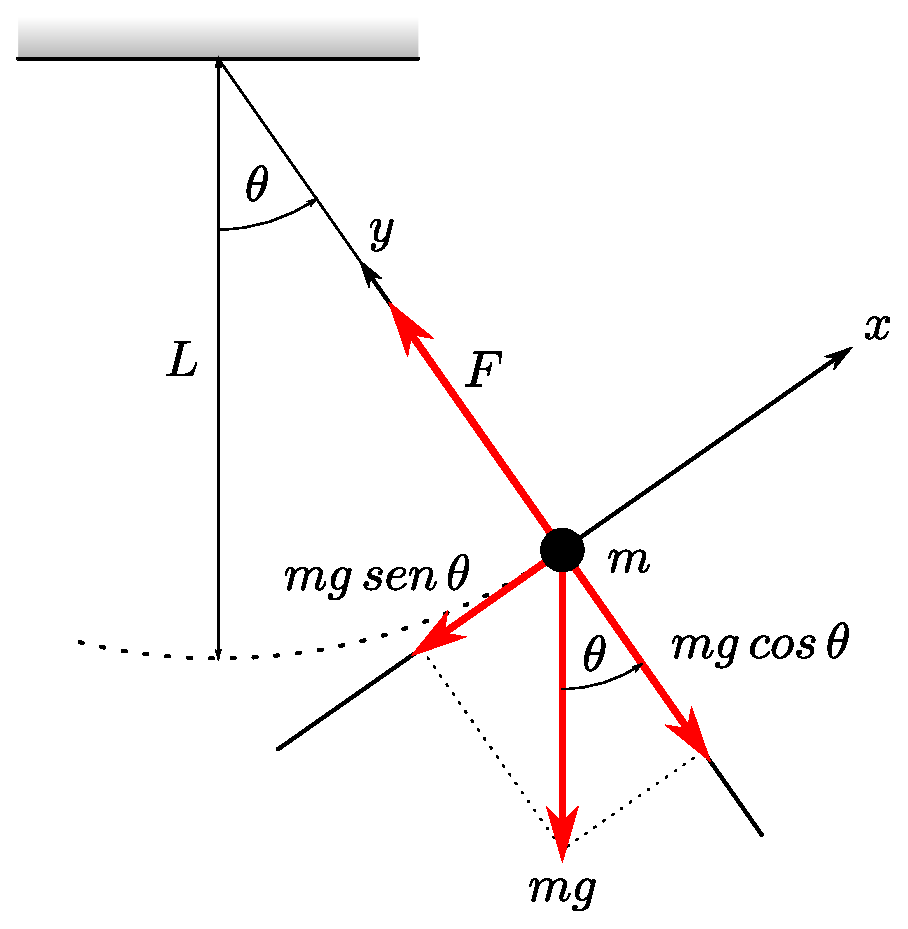
\includegraphics[width=0.38\textwidth]{resources/f1.eps}
\caption{Péndulo simple idealizado.}
\label{figura1}
\source{Física Universitaria Volumen I (p. 454), \\
Young, Hugh D. y Freedman, Roger A., 2013, Pearson.}
\end{figure}

En la \textbf{Figura \ref{figura1}} se detallan las fuerzas que actúan sobre la
masa ($m$) en cualquier instante del movimiento, estas fuerzas son: La tensión
($F$) de la cuerda y la fuerza de gravedad ($mg$), que se descompone en función
del ángulo desplazado ($\theta$), en una componente normal ($mg\, cos\, \theta$)
y una componente tangencial ($mg\, sen\, \theta$) \cite{GUIA}.

Aplicando la segunda ley de \emph{Newton} en la dirección tangencial, se
obtiene:

\begin{equation*}
    -mg\, sen\, (\theta) = m\, a_t
\label{segundaley}
\end{equation*}
\vspace{0.10cm}

La aceleración en la dirección tangencial es:

\begin{equation*}
    a_t = \frac{d^2 S}{dt^2}
\end{equation*}
\vspace{0.10cm}

Donde $S$ es la longitud del arco o trayectoria circular, cuya relación con el
ángulo $\theta$ y la longitud de la cuerda $L$ es:

\begin{equation*}
    S = \theta\, L
\end{equation*}
\vspace{0.10cm}

Por tanto:

\begin{equation*}
    \frac{d^2 \theta}{dt^2} + \frac{g}{L} sen\, (\theta) = 0
\end{equation*}
\vspace{0.10cm}

Si se consideran tan solo oscilaciones de pequeña amplitud, de modo que el
ángulo $\theta$ sea siempre suficientemente pequeño, entonces el valor del
$sen\, (\theta)$ será muy próximo al valor de $\theta$ expresado en radianes
($sen\, (\theta) \cong \theta$, para $\theta$ suficientemente pequeño), como
se aprecia en el \textbf{Cuadro \ref{cuadro1}} \cite{WIKI1}.

\begin{table}[!h]
\begin{center}
\begin{tabular}{|>{\centering}m{0.50cm}<{\centering}
                |>{\centering}m{1.25cm}<{\centering}
                |>{\centering}m{1.25cm}<{\centering}
                |>{\centering}m{2.50cm}<{\centering}|
                |>{\centering}m{0.50cm}<{\centering}
                |>{\centering}m{1.25cm}<{\centering}
                |>{\centering}m{1.25cm}<{\centering}
                |>{\centering}m{2.50cm}<{\centering}|}
\hline
$\theta [^\circ]$ & $\theta [rad]$ & $sen\, (\theta)$ & diferencia (\%) &
$\theta [^\circ]$ & $\theta [rad]$ & $sen\, (\theta)$ & diferencia (\%)
    \tabularnewline \hline
\hline
 0 & 0.00000 & 0.00000 & 0.00 & 15 & 0.26180 & 0.25882 & 1.15
    \tabularnewline \hline
 2 & 0.03491 & 0.03490 & 0.02 & 20 & 0.34907 & 0.34202 & 2.06
    \tabularnewline \hline
 5 & 0.08727 & 0.08716 & 0.13 & 25 & 0.43633 & 0.42262 & 3.25
    \tabularnewline \hline
10 & 0.17453 & 0.17365 & 0.51 & 30 & 0.52360 & 0.50000 & 4.72
    \tabularnewline \hline
\end{tabular}
\caption{Comparación entre el valor del ángulo y su función seno.}
\label{cuadro1}
\source{Adaptado de péndulo simple (Wikipedia).}
\end{center}
\end{table}

La ecuación anterior se reduce a:

\begin{equation*}
    \frac{d^2 \theta}{dt^2} + \frac{g}{L} \theta = 0
\label{oscilador}
\end{equation*}
\vspace{0.10cm}

La \textbf{Ecuación \ref{oscilador}} corresponde a un \textbf{oscilador armónico
simple} cuya solución general es:

\begin{equation*}
    \theta(t) = A\, cos\, (\omega\, t + \phi)
\end{equation*}
\vspace{0.10cm}

Donde $A$ representa el máximo desplazamiento angular de $\theta$, $\omega$ es
la frecuencia angular, y $\phi$ el desfase. Tanto la magnitud $A$, como $\phi$
son dos constantes determinadas por las condiciones iniciales.

La frecuencia angular ($\omega$) esta determinada por:

\begin{equation*}
    \omega = \sqrt{\frac{g}{L}}
\end{equation*}
\vspace{0.10cm}

Considerando que $\omega = 2\pi / T$, el periodo de oscilación para el péndulo
simple es:

\begin{equation}
    T = 2\pi\, \sqrt{\frac{L}{g}} = \frac{2\pi}{\sqrt{g}} \sqrt{L}
\label{periodo}
\end{equation}
\vspace{0.10cm}

Para el experimento se comprobará la relación funcional entre la longitud de la
cuerda establecida ($L$), y el periodo ($T$), establecida por la
\textbf{Ecuación \ref{periodo}}. Finalmente se determinará el valor de la
gravedad ($g$) en Cochabamba, despejando la variable ($g$).

\section{Método experimental}

\begin{figure}
\centering

\includegraphics[width=0.70\textwidth]{resources/f2.eps}
\caption{Montaje para el experimento.}
\label{figura2}
\source{Fotografía propia.}
\end{figure}

Para facilitar la medición, se ha armado el equipo mostrado en la
\textbf{Figura \ref{figura2}}, el cual consta de un barra horizontal
previamente nivelada, a la cual se ha sujetado un transportador para que la
oscilación no exceda los $10^\circ$. Una vez montado el soporte, se escogió una
moneda de colección atada a hilo que se haría oscilar.

Se escoge un valor de longitud ($L$) y se registrará la cantidad de tiempo
que requiere el péndulo para hacer 10 oscilaciones completas.

Una vez medidos los datos para 5 valores distintos de longitud ($L$), se
procederá a calcular el periodo ($T$) con la siguiente ecuación:

\begin{equation}
    T = \frac{t}{10}
\label{periodo10}
\end{equation}
\vspace{0.10cm}

Luego se procederá a graficar la relación longitud ($L$) vs. periodo ($T$), para
realizar primeramente la linealización de la curva por logaritmos, y luego el
calculo de la recta por el método de los mínimos cuadrados, posteriormente
hallar la relación funcional entre las variables.

Finalizando con el calculo del valor de la gravedad, a partir de la
\textbf{Ecuación \ref{periodo}}:

\begin{equation*}
    a = \frac{2 \pi}{\sqrt{g}}
\end{equation*}
\vspace{0.10cm}

Donde $a$ es uno de los parámetros de la curva hallada.

Despejando $g$, se obtiene:

\begin{equation}
    g = \frac{4 \pi^2}{a^2}
\label{gravedad}
\end{equation}
\vspace{0.10cm}

\textbf{Datos tomados en el experimento:} \\

En el \textbf{Cuadro \ref{cuadro2}}, se pueden ver los valores tomados del 
experimento, tanto la longitud como el tiempo de 10 oscilaciones, además del
valor del periodo resultante.

\begin{table}[!h]
\begin{center}
\begin{tabular}{|c||>{\centering}m{2.4cm}<{\centering}|
                  |>{\centering}m{2.4cm}<{\centering}|
                  |>{\centering}m{2.4cm}<{\centering}|}
\hline
$i$ & $L_i [m]$ & $t_{1i} [s]$ & $T_i [s]$
    \tabularnewline \hline \hline
 1 & 0.630 & 15.75 & 1.5750 \tabularnewline \hline
 2 & 0.580 & 15.25 & 1.5250 \tabularnewline \hline
 3 & 0.525 & 14.74 & 1.4740 \tabularnewline \hline
 4 & 0.480 & 13.96 & 1.3960 \tabularnewline \hline
 5 & 0.425 & 13.13 & 1.3130 \tabularnewline \hline
\end{tabular}
\caption{Mediciones de tiempo en función de la longitud del péndulo.}
\label{cuadro2}
\source{Elaboración propia.}
\end{center}
\end{table}

\begin{figure}
\centering
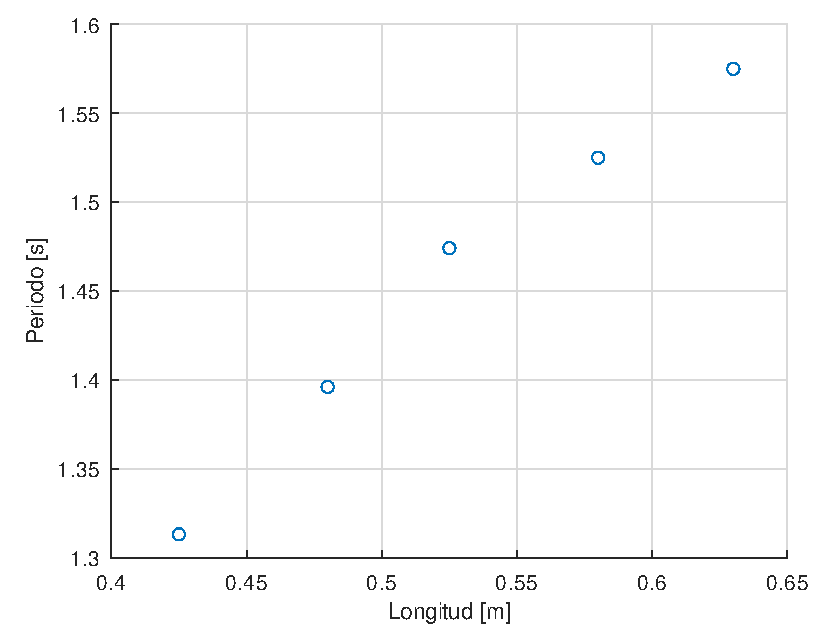
\includegraphics[width=0.75\textwidth]{resources/o1.1.eps}
\caption{Gráfica de longitud vs periodo.}
\label{figura3}
\source{Elaboración propia.}
\end{figure}

\section{Resultados}

A partir de los datos obtenidos se calculó el periodo de oscilación ($T$) para
los valores de longitud ($L$), con los que se generó la gráfica de la
\textbf{Figura \ref{figura3}}.

Posteriormente se linealizó la curva por medio de logaritmos, y se calculó la
recta de mejor ajuste por el método de los mínimos cuadrados, resultando los
siguientes valores:

\begin{equation*}
    A = (0.68 \pm 0.02) [u]; 2.70\%
\end{equation*}
\begin{equation*}
    B = (0.46 \pm 0.03) [u]; 5.90\%
\end{equation*}
\vspace{0.10cm}

Siendo su coeficiente de correlación ($r$):

\begin{equation*}
    r = 0.9948
\end{equation*}
\vspace{0.10cm}

Con los valores hallados, se calculan los valores originales de la curva,
resultando:

\begin{equation*}
    a = (1.96 \pm 0.03) [s/\sqrt{m}]; 1.81\%
\end{equation*}
\begin{equation*}
    b = (0.46 \pm 0.03) [u]; 5.90\%
\end{equation*}
\vspace{0.10cm}

Resultando el modelo de ajuste:

\begin{equation*}
    T = 1.96\,L^{0.46}
\end{equation*}
\vspace{0.10cm}

Por tanto la relación funcional aproximada entre $T$ y $L$, es:

\begin{center}
\begin{tabular}{|>{\centering}m{9.2cm}<{\centering}|}
\hline
\textbf{Resultado} 
\tabularnewline \hline
\\
$T \propto \sqrt{L}$ \tabularnewline
\\
\hline
\end{tabular}
\end{center}
\vspace{0.10cm}

Verificándose el comportamiento establecido por la
\textbf{Ecuación \ref{periodo}}.

Para el calculo de la gravedad ($g$) se utiliza la
\textbf{Ecuación \ref{gravedad}}, resultando:

\begin{center}
\begin{tabular}{|>{\centering}m{9.2cm}<{\centering}|}
\hline
\textbf{Resultado} 
\tabularnewline \hline
\\
$g = (10.23 \pm 0.37) [m/s^2]; 3.63\%$ \tabularnewline
\\
\hline
\end{tabular}
\end{center}
\vspace{0.10cm}

\section{Discusión}

Considerando la discrepancia entre el valor nominal de la gravedad 
$g = (9.78 \pm 0.02)[m/s^2]$ y el resultado hallado, se considera que la baja
cantidad de datos, además que la toma de una única repetición, esta afectando
mucho la medición.

Se recomienda realizar el experimento con mas de 5 datos, y con mayor numero de
repeticiones, para mejorar la precisión del experimento.

Cosa que no se realizó en este por la falta del tiempo necesario para la toma
de datos.

\section{Conclusiones}

Se verificaron las ecuaciones planteadas en la introducción, así como la
ecuación de un oscilador armónico simple.

También se calculó el valor de la gravedad, a pesar de la notoria discrepancia
con el valor teórico.

\begin{thebibliography}{99}

\bibitem{Young&Freedman} Young, Hugh D. y Freedman, Roger A. (2013).\\
Física Universitaria. Volumen 1.\\
13va Edición.\\
Capitulo 14.

\bibitem{GUIA} Departamento de Física - UMSS.\\
Laboratorio de Física Básica II.\\
Guía - Cartilla de laboratorio.\\
Gestión I/2020.

\bibitem{WIKI1} Péndulo simple \\
Extraído el 27 de Abril del 2021, de: \\
\url{https://es.wikipedia.org/wiki/P%C3%A9ndulo_simple}.

\end{thebibliography}

\newpage
\section*{Apéndice A: Cálculos realizados en \emph{Octave}}

A continuación se presenta los cálculos realizados en el programa \emph{Octave}
para la generación de las gráficas, la linealización de la curva, el calculo
de los mínimos cuadrados y el valor de la gravedad.

\begin{shaded}
\begin{alltt}
\footnotesize
\# Datos importados (i1.csv):
\input{resources/i1.csv}
\normalsize
\end{alltt}
\end{shaded}

\begin{shaded}
\begin{alltt}
\footnotesize
\# Comandos ejecutados (o1.m):
\input{../../octave/graficar.m}
\input{../../octave/minimoscuadrados.m}
\input{resources/o1.m}
\normalsize
\end{alltt}
\end{shaded}

\begin{shaded}
\begin{alltt}
\footnotesize
\# Salida del programa (o1.out):
\input{resources/o1.out}
\normalsize
\end{alltt}
\end{shaded}

\end{document}

